% !Mode:: "TeX:UTF-8"

\BiChapter{多尺度网络在求解椭圆方程中的应用}{}

这里我们应用带有激活函数为$\mathrm{Phi}(x)$的多尺度网络来求解复杂的椭圆型方程。具体实验包括求解具有宽频率范围、变系数、环形区域上和多孔的立方区域上的椭圆方程。通过这些实验,我们令人信服地证明了多尺度网络是一种有效且易于实现的求解复杂椭圆方程的无网格方法。

\BiSection{宽频域振荡的椭圆方程}{}

求解椭圆方程\ref{prob1},其中参数选取为$a(x)=1$,$c(x)=0$,求解区域为$\Omega = [-1, 1]^d$,右端项表达式为
\begin{equation}
f(x) = \sum_{i=1}^{d}  4 \mu^2 x_i^2 \sin(\mu x_i^2) - 2 \mu \cos(\mu x_i^2)
\end{equation}
方程的精确解为
\begin{equation}
u(x) = \sum_{i=1}^{d} \sin(\mu x_i^2)
\end{equation}
对应的边界条件由精确解生成。

每步中我们随机在区域$[-1, 1]^d$内选取$5000$个均匀分布的积分点,在边界上生成$4000$个均匀分布的积分点。这个问题的特殊之处在于,精确解虽然是高频振荡的,但是它没有固定的频率,而是有一个广泛的频率范围。对于$\mu=15$,二维情况下问题的精确解和两种网络结构下的近似解如图\ref{func3}所示。图中指出,多尺度网络得到的解很好地捕捉到不同尺度的振荡。例如,在红圈所示区域,普通的全连接网络没有捕捉到解的振荡,而多尺度网络的解很好地展示出了振荡的形态。在四个角处的振荡也出现了类似的行为。

\begin{figure}[htbp]
\centering
\subfigure[exact]{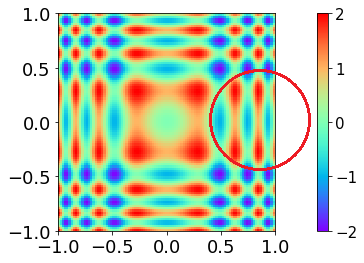
\includegraphics[width=0.3\linewidth]{\fpath exp4/M20E2d_samp}}
\subfigure[normal]{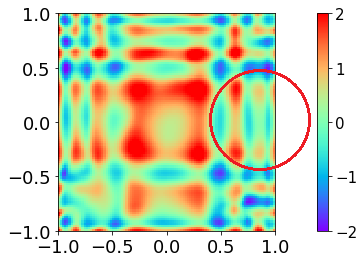
\includegraphics[width=0.3\linewidth]{\fpath exp4/M20N2d_samp}}
\subfigure[Mscale]{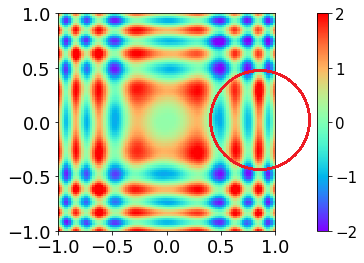
\includegraphics[width=0.3\linewidth]{\fpath exp4/M20S2d_samp}}
\caption{二维情况下椭圆方程的精确解和数值解图像}
\label{func3}
\end{figure}

求解结果如图\ref{e4},图中画出了求解方程的误差随迭代步数下降的图像。在求解二维和三维的方程中,多尺度网络都表现出了明显的优势。

\begin{figure}[htbp]
\centering
\subfigure[二维情况]{\includegraphics[width=0.35\linewidth]{\fpath E42d}}
\subfigure[三维情况]{\includegraphics[width=0.35\linewidth]{\fpath E43d}}
\caption{二维和三维情况下两种网络结构的表现}
\label{e4}
\end{figure}

\BiSection{环形区域上的的椭圆方程}{}

求解椭圆方程\ref{prob1},其中参数选取为$a(x)=1$,$c(x)=0$,求解区域为一个以原点为中心的圆环,内径为$1$,外径为$3$。方程的右端项表达式为
\begin{equation}
f(x) = \mu^2 J_0(\mu |x - x_0|)
\end{equation}
其中$J_0$是Bessel函数,方程的精确解为
\begin{equation}
u(x) = J_0(\mu |x - x_0|)
\end{equation}
对应的边界条件由精确解生成。位移选取为$x_0 = (0.5, 0)$,参数选取为$\mu=5$和$\mu=10$分别实验。

每步中我们随机在区域内选取$5000$个均匀分布的积分点,在边界上生成$4000$个均匀分布的积分点。问题的精确解和两种网络结构下的近似解如图\ref{func4-m5}和图\ref{func4-m10}所示。图中用黑色圆圈标记的区域表示解在此处有最大的振幅,正常的全连接网络完全不能刻画振荡,而多尺度网络在这两种情况下都可以得到和精确解类似的效果。

同样,如图\ref{e6}所示,图中画出了求解方程的误差随迭代步数下降的图像。在迭代同样的步数后,多尺度网络的误差更小。

\begin{figure}[htbp]
\centering
\subfigure[exact]{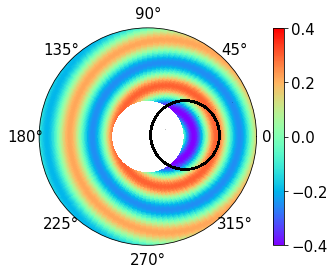
\includegraphics[width=0.3\linewidth]{\fpath exp6/U2M5E_samp}}
\subfigure[normal]{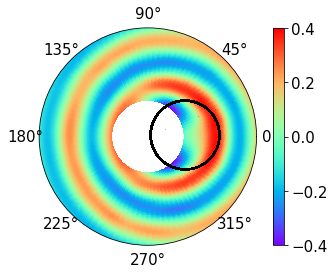
\includegraphics[width=0.3\linewidth]{\fpath exp6/U2M5N_samp}}
\subfigure[Mscale]{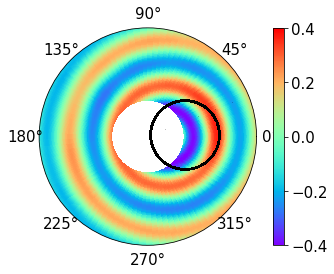
\includegraphics[width=0.3\linewidth]{\fpath exp6/U2M5S_samp}}
\caption{$\mu=5$情况下椭圆方程的精确解和数值解图像}
\label{func4-m5}
\end{figure}

\begin{figure}[htbp]
\centering
\subfigure[exact]{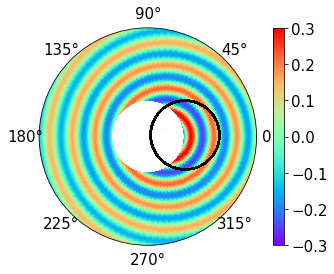
\includegraphics[width=0.3\linewidth]{\fpath exp6/U2M10E_samp}}
\subfigure[normal]{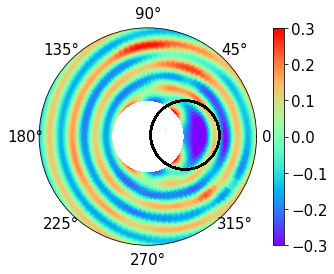
\includegraphics[width=0.3\linewidth]{\fpath exp6/U2M10N_samp}}
\subfigure[Mscale]{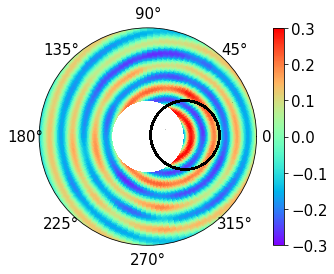
\includegraphics[width=0.3\linewidth]{\fpath exp6/U2M10S_samp}}
\caption{$\mu=10$情况下椭圆方程的精确解和数值解图像}
\label{func4-m10}
\end{figure}

\begin{figure}[htbp]
\centering
\subfigure[$\mu=5$]{\includegraphics[width=0.35\linewidth]{\fpath E6M5}}
\subfigure[$\mu=10$]{\includegraphics[width=0.35\linewidth]{\fpath E6M10}}
\caption{不同参数下两种网络结构的表现}
\label{e6}
\end{figure}

\BiSection{有孔区域上的的椭圆方程}{}

这里我们考虑如下两个区域:

{\bf 区域1:} 方形区域$[-1, 1]^2$内有三个圆形的孔。三个圆孔的中心分别为$(-0.5,-0.5)$、$(0.5,0.5)$和$(0.5,-0.5)$,半径分别为$0.1$、$0.2$和$0.2$。在训练过程中,每步我们随机在区域内选取$5000$个均匀分布的积分点,在方形区域的边界上生成$3000$个积分点,每个大圆孔的边界上生成$800$个积分点,每个小圆孔的边界上生成$400$个积分点。

{\bf 区域2} 方形区域$[-1, 1]^2$内有四个孔。三个圆形孔的中心分别为$(-0.6,-0.6)$,$(0.3,-0.3)$和$(0.6,0.6)$,半径分别为$0.3$,$0.6$和$0.3$。椭圆形孔由方程$16(x+0.5)^2+64(y-0.5)^2=1$表示。每步我们随机在区域内选取$5000$个均匀分布的积分点,外部边界、大圆孔边界、小圆孔边界和椭圆孔边界生成的积分点数量分别为$2400$、$1100$、$550$和$400$。

求解椭圆方程\ref{prob1},其中参数选取为$a(x)=1$,$c(x)=0$。方程的右端项表达式为
\begin{equation}
f(x) = 2 \mu^2 \sin \mu x_1 \; \sin \mu x_2
\end{equation}
方程的精确解为
\begin{equation}
u(x) = \sin \mu x_1 \sin \mu x_2
\end{equation}
对应的边界条件由精确解生成。其中的参数选取为$\mu = 7 \pi$。

问题的精确解和两种网络结构下的近似解如图\ref{func4-m5}和图\ref{func4-m10}所示。显然,多尺度网络能更好地刻画精确解中的振荡。

\begin{figure}[htbp]
\centering
\subfigure[exact]{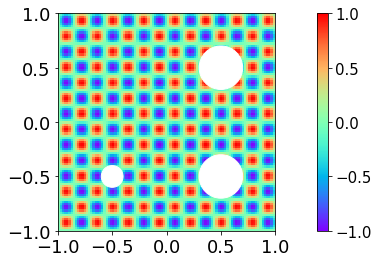
\includegraphics[width=0.3\linewidth]{\fpath exp7/R1M7E_samp}}
\subfigure[normal]{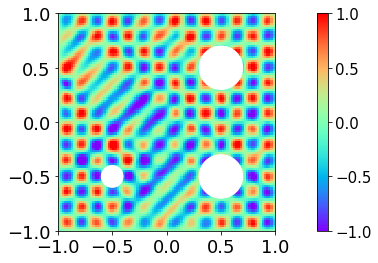
\includegraphics[width=0.3\linewidth]{\fpath exp7/R1M7N_samp}}
\subfigure[Mscale]{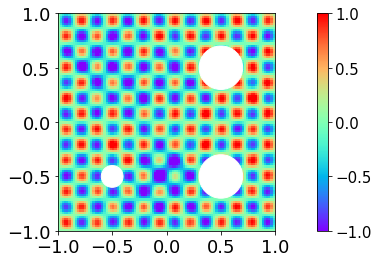
\includegraphics[width=0.3\linewidth]{\fpath exp7/R1M7S_samp}}
\caption{区域1上椭圆方程的精确解和数值解图像}
\label{func5-r1}
\end{figure}

\begin{figure}[htbp]
\centering
\subfigure[exact]{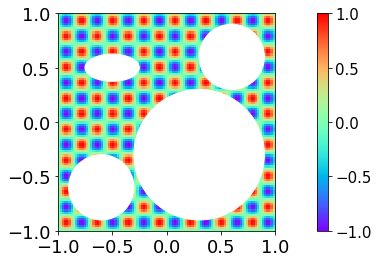
\includegraphics[width=0.3\linewidth]{\fpath exp7/R2M7E_samp}}
\subfigure[normal]{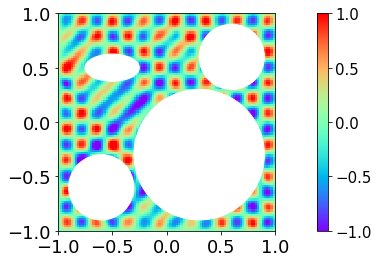
\includegraphics[width=0.3\linewidth]{\fpath exp7/R2M7N_samp}}
\subfigure[Mscale]{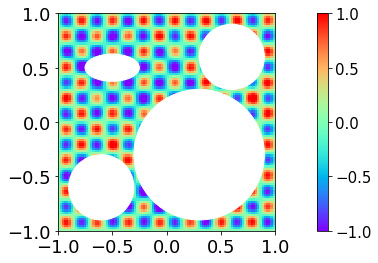
\includegraphics[width=0.3\linewidth]{\fpath exp7/R2M7S_samp}}
\caption{区域2上椭圆方程的精确解和数值解图像}
\label{func5-r2}
\end{figure}

同样,如图\ref{e7}所示,图中画出了求解方程的误差随迭代步数下降的图像,多尺度网络的误差下降速度更快,精度也更高。

\begin{figure}[htbp]
\centering
\subfigure[区域1]{\includegraphics[width=0.35\linewidth]{\fpath E7R1}}
\subfigure[区域2]{\includegraphics[width=0.35\linewidth]{\fpath E7R2}}
\caption{两种区域下不同网络结构的表现}
\label{e7}
\end{figure}

\BiSection{多孔区域上的的椭圆方程}{}

为了验证多尺度网络求解复杂区域上椭圆方程的能力,我们考虑了一个三维立方体$[-1,1]^3$,内部移除了125个孔,如图\ref{func6},这些球形孔的球心位于正方体内部的均匀网格$\{-0.8, -0.4, 0, 0.4, 0.8\}^3$上。这些孔的半径是从范围在$[0, 0.15]$中的均匀分布随机抽样产生,这样可以保证各个孔之间没有相交。在训练过程中,每步我们随机在区域内选取$5000$个均匀分布的积分点,外边界生成2500个积分点,内部的孔上1500个(每个孔12个)积分点。

\begin{figure}[htbp]
\centering
\includegraphics[width=0.4\linewidth]{\fpath holes}
\caption{多孔区域示意图,蓝色表示在区域内挖去的部分}
\label{func6}
\end{figure}

求解椭圆方程\ref{prob1},其中参数选取为$a(x)=1$,$c(x)=0$,$\mu=7\pi$。我们测试如下三组示例,它们对应的精确解分别为
\begin{enumerate}
\item  示例 1: $ u(x) = \sin \mu x_1 \sin \mu x_2 \sin \mu x_3 $
\item  示例 2: $ u(x) = {\mathrm{e}}^{\sin \mu x_1 + \sin \mu x_2 + \sin \mu x_3} $
\item  示例 3: $ u(x) = \mathrm{e}^{ \sin \mu x_1 \sin \mu x_2 \sin \mu x_3 } $
\end{enumerate}
对应的边界条件和右端项由精确解生成。

\begin{figure}[htbp]
\centering
\subfigure[示例 1]{\includegraphics[width=0.3\linewidth]{\fpath E8U1}}
\subfigure[示例 2]{\includegraphics[width=0.3\linewidth]{\fpath E8U2}}
\subfigure[示例 3]{\includegraphics[width=0.3\linewidth]{\fpath E8U3}}
\caption{三个示例中不同网络结构的表现}
\label{e8}
\end{figure}

计算结果如图\ref{e8}所示,在三维区域上,我们难以画出精确解和近似解的图像,这里只给出了误差随迭代步数变化的图像。对于这三种情况,正常的全连通网络结构对于此类复杂问题根本不收敛,在迭代的过程中误差几乎不下降,而多尺度网络虽然在计算开始时误差上升,但是在一定的步数之后就可以明显达到更小的误差。

\BiSection{变系数椭圆方程}{}

求解椭圆方程\ref{prob1},其中参数选取为$a(x)=1$,方程的右端项表达式为
\begin{equation}
f(x) = (\mu_1^2 + \mu_2^2 + \mu_3^2 + x_1^2 + 2 x_2^2 + 3 x_3^2) \sin(\mu_1 x_1) \sin(\mu_2 x_2) \sin(\mu_3 x_3)
\end{equation}
系数表达式为
\begin{equation}
c(x) = (x_1^2 + 2 x_2^2 + 3 x_3^2)
\end{equation}
方程的精确解为
\begin{equation}
u(x) = \sin(\mu_1 x_1) \sin(\mu_2 x_2) \sin(\mu_3 x_3)
\end{equation}
对应的边界条件由精确解生成。我们选取各向异性的参数,其中$\mu_1=15, \mu_2=20, \mu_3=25$。

每步中我们随机在求解区域$[-1, 1]^d$内选取$5000$个均匀分布的积分点,在边界上生成$4000$个均匀分布的积分点。

\begin{figure}[htbp]
\centering
\includegraphics[width=0.4\linewidth]{\fpath E5}
\caption{两种网络结构的表现}
\label{e5}
\end{figure}

如图\ref{e5}所示,在训练过程中,多尺度网络的误差显著衰减,而正常的全连接网络误差几乎保持不变。多尺度网络以更高的精度更快地解决了问题。
